% Created by tikzDevice version 0.9 on 2016-01-13 23:40:06
% !TEX encoding = UTF-8 Unicode
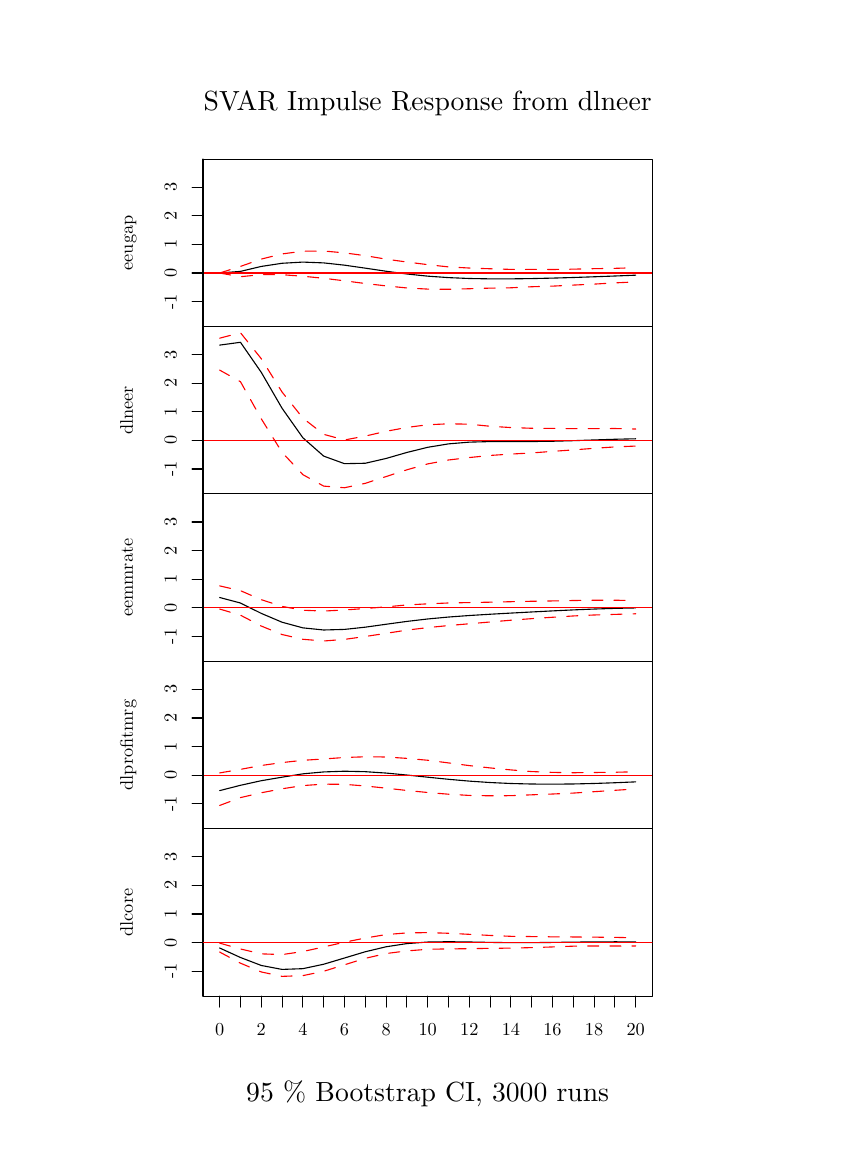
\begin{tikzpicture}[x=1pt,y=1pt]
\definecolor{fillColor}{RGB}{255,255,255}
\path[use as bounding box,fill=fillColor,fill opacity=0.00] (0,0) rectangle (289.08,397.48);
\begin{scope}
\path[clip] ( 63.36,289.48) rectangle (225.72,349.96);
\definecolor{drawColor}{RGB}{0,0,0}

\path[draw=drawColor,line width= 0.4pt,line join=round,line cap=round] ( 69.37,308.82) --
	( 76.89,309.41) --
	( 84.41,311.20) --
	( 91.92,312.34) --
	( 99.44,312.77) --
	(106.96,312.48) --
	(114.47,311.66) --
	(121.99,310.58) --
	(129.51,309.46) --
	(137.02,308.47) --
	(144.54,307.69) --
	(152.06,307.16) --
	(159.57,306.84) --
	(167.09,306.71) --
	(174.61,306.71) --
	(182.12,306.81) --
	(189.64,306.98) --
	(197.16,307.20) --
	(204.67,307.46) --
	(212.19,307.74) --
	(219.71,308.04);
\end{scope}
\begin{scope}
\path[clip] ( 31.68,289.48) rectangle (257.40,349.96);
\definecolor{drawColor}{RGB}{0,0,0}

\node[text=drawColor,anchor=base,inner sep=0pt, outer sep=0pt, scale=  0.66] at (144.54,259.38) {xy{\$}x};

\node[text=drawColor,rotate= 90.00,anchor=base,inner sep=0pt, outer sep=0pt, scale=  0.66] at ( 38.02,319.72) {eeugap};
\end{scope}
\begin{scope}
\path[clip] (  0.00,  0.00) rectangle (289.08,397.48);
\definecolor{drawColor}{RGB}{0,0,0}

\path[draw=drawColor,line width= 0.4pt,line join=round,line cap=round] ( 63.36,298.49) -- ( 63.36,349.97);

\path[draw=drawColor,line width= 0.4pt,line join=round,line cap=round] ( 63.36,298.49) -- ( 59.40,298.49);

\path[draw=drawColor,line width= 0.4pt,line join=round,line cap=round] ( 63.36,308.82) -- ( 59.40,308.82);

\path[draw=drawColor,line width= 0.4pt,line join=round,line cap=round] ( 63.36,319.16) -- ( 59.40,319.16);

\path[draw=drawColor,line width= 0.4pt,line join=round,line cap=round] ( 63.36,329.49) -- ( 59.40,329.49);

\path[draw=drawColor,line width= 0.4pt,line join=round,line cap=round] ( 63.36,339.83) -- ( 59.40,339.83);

\node[text=drawColor,rotate= 90.00,anchor=base,inner sep=0pt, outer sep=0pt, scale=  0.66] at ( 53.86,298.49) {-1};

\node[text=drawColor,rotate= 90.00,anchor=base,inner sep=0pt, outer sep=0pt, scale=  0.66] at ( 53.86,308.82) {0};

\node[text=drawColor,rotate= 90.00,anchor=base,inner sep=0pt, outer sep=0pt, scale=  0.66] at ( 53.86,319.16) {1};

\node[text=drawColor,rotate= 90.00,anchor=base,inner sep=0pt, outer sep=0pt, scale=  0.66] at ( 53.86,329.49) {2};

\node[text=drawColor,rotate= 90.00,anchor=base,inner sep=0pt, outer sep=0pt, scale=  0.66] at ( 53.86,339.83) {3};
\end{scope}
\begin{scope}
\path[clip] ( 63.36,289.48) rectangle (225.72,349.96);
\definecolor{drawColor}{RGB}{255,0,0}

\path[draw=drawColor,line width= 0.4pt,line join=round,line cap=round] ( 63.36,308.82) -- (225.72,308.82);

\path[draw=drawColor,line width= 0.4pt,dash pattern=on 4pt off 4pt ,line join=round,line cap=round] ( 69.37,308.82) --
	( 76.89,311.21) --
	( 84.41,313.85) --
	( 91.92,315.72) --
	( 99.44,316.70) --
	(106.96,316.78) --
	(114.47,316.10) --
	(121.99,315.09) --
	(129.51,313.83) --
	(137.02,312.79) --
	(144.54,311.85) --
	(152.06,311.03) --
	(159.57,310.62) --
	(167.09,310.36) --
	(174.61,310.13) --
	(182.12,310.12) --
	(189.64,310.09) --
	(197.16,310.22) --
	(204.67,310.39) --
	(212.19,310.51) --
	(219.71,310.74);

\path[draw=drawColor,line width= 0.4pt,dash pattern=on 4pt off 4pt ,line join=round,line cap=round] ( 69.37,308.82) --
	( 76.89,307.48) --
	( 84.41,308.24) --
	( 91.92,308.21) --
	( 99.44,307.66) --
	(106.96,306.92) --
	(114.47,306.00) --
	(121.99,305.03) --
	(129.51,304.17) --
	(137.02,303.42) --
	(144.54,303.01) --
	(152.06,302.94) --
	(159.57,303.14) --
	(167.09,303.36) --
	(174.61,303.48) --
	(182.12,303.86) --
	(189.64,304.08) --
	(197.16,304.46) --
	(204.67,304.81) --
	(212.19,305.26) --
	(219.71,305.60);
\end{scope}
\begin{scope}
\path[clip] (  0.00,  0.00) rectangle (289.08,397.48);
\definecolor{drawColor}{RGB}{0,0,0}

\path[draw=drawColor,line width= 0.4pt,line join=round,line cap=round] ( 63.36,289.48) --
	(225.72,289.48) --
	(225.72,349.96) --
	( 63.36,349.96) --
	( 63.36,289.48);
\end{scope}
\begin{scope}
\path[clip] ( 63.36,228.99) rectangle (225.72,289.48);
\definecolor{drawColor}{RGB}{0,0,0}

\path[draw=drawColor,line width= 0.4pt,line join=round,line cap=round] ( 69.37,282.77) --
	( 76.89,283.79) --
	( 84.41,272.93) --
	( 91.92,259.95) --
	( 99.44,249.29) --
	(106.96,242.66) --
	(114.47,239.93) --
	(121.99,240.08) --
	(129.51,241.81) --
	(137.02,243.98) --
	(144.54,245.84) --
	(152.06,247.08) --
	(159.57,247.71) --
	(167.09,247.91) --
	(174.61,247.92) --
	(182.12,247.93) --
	(189.64,248.03) --
	(197.16,248.24) --
	(204.67,248.50) --
	(212.19,248.75) --
	(219.71,248.92);
\end{scope}
\begin{scope}
\path[clip] ( 31.68,228.99) rectangle (257.40,289.48);
\definecolor{drawColor}{RGB}{0,0,0}

\node[text=drawColor,anchor=base,inner sep=0pt, outer sep=0pt, scale=  0.66] at (144.54,198.89) {xy{\$}x};

\node[text=drawColor,rotate= 90.00,anchor=base,inner sep=0pt, outer sep=0pt, scale=  0.66] at ( 38.02,259.23) {dlneer};
\end{scope}
\begin{scope}
\path[clip] (  0.00,  0.00) rectangle (289.08,397.48);
\definecolor{drawColor}{RGB}{0,0,0}

\path[draw=drawColor,line width= 0.4pt,line join=round,line cap=round] ( 63.36,238.00) -- ( 63.36,289.48);

\path[draw=drawColor,line width= 0.4pt,line join=round,line cap=round] ( 63.36,238.00) -- ( 59.40,238.00);

\path[draw=drawColor,line width= 0.4pt,line join=round,line cap=round] ( 63.36,248.33) -- ( 59.40,248.33);

\path[draw=drawColor,line width= 0.4pt,line join=round,line cap=round] ( 63.36,258.67) -- ( 59.40,258.67);

\path[draw=drawColor,line width= 0.4pt,line join=round,line cap=round] ( 63.36,269.00) -- ( 59.40,269.00);

\path[draw=drawColor,line width= 0.4pt,line join=round,line cap=round] ( 63.36,279.34) -- ( 59.40,279.34);

\node[text=drawColor,rotate= 90.00,anchor=base,inner sep=0pt, outer sep=0pt, scale=  0.66] at ( 53.86,238.00) {-1};

\node[text=drawColor,rotate= 90.00,anchor=base,inner sep=0pt, outer sep=0pt, scale=  0.66] at ( 53.86,248.33) {0};

\node[text=drawColor,rotate= 90.00,anchor=base,inner sep=0pt, outer sep=0pt, scale=  0.66] at ( 53.86,258.67) {1};

\node[text=drawColor,rotate= 90.00,anchor=base,inner sep=0pt, outer sep=0pt, scale=  0.66] at ( 53.86,269.00) {2};

\node[text=drawColor,rotate= 90.00,anchor=base,inner sep=0pt, outer sep=0pt, scale=  0.66] at ( 53.86,279.34) {3};
\end{scope}
\begin{scope}
\path[clip] ( 63.36,228.99) rectangle (225.72,289.48);
\definecolor{drawColor}{RGB}{255,0,0}

\path[draw=drawColor,line width= 0.4pt,line join=round,line cap=round] ( 63.36,248.33) -- (225.72,248.33);

\path[draw=drawColor,line width= 0.4pt,dash pattern=on 4pt off 4pt ,line join=round,line cap=round] ( 69.37,285.27) --
	( 76.89,287.24) --
	( 84.41,277.86) --
	( 91.92,265.82) --
	( 99.44,256.40) --
	(106.96,250.53) --
	(114.47,248.49) --
	(121.99,249.90) --
	(129.51,251.62) --
	(137.02,253.02) --
	(144.54,253.99) --
	(152.06,254.33) --
	(159.57,254.20) --
	(167.09,253.45) --
	(174.61,252.98) --
	(182.12,252.72) --
	(189.64,252.69) --
	(197.16,252.57) --
	(204.67,252.57) --
	(212.19,252.63) --
	(219.71,252.45);

\path[draw=drawColor,line width= 0.4pt,dash pattern=on 4pt off 4pt ,line join=round,line cap=round] ( 69.37,273.74) --
	( 76.89,269.55) --
	( 84.41,256.15) --
	( 91.92,244.03) --
	( 99.44,235.96) --
	(106.96,231.82) --
	(114.47,231.23) --
	(121.99,232.82) --
	(129.51,235.27) --
	(137.02,237.71) --
	(144.54,239.84) --
	(152.06,241.26) --
	(159.57,242.14) --
	(167.09,242.90) --
	(174.61,243.40) --
	(182.12,243.80) --
	(189.64,244.38) --
	(197.16,244.90) --
	(204.67,245.48) --
	(212.19,245.98) --
	(219.71,246.29);
\end{scope}
\begin{scope}
\path[clip] (  0.00,  0.00) rectangle (289.08,397.48);
\definecolor{drawColor}{RGB}{0,0,0}

\path[draw=drawColor,line width= 0.4pt,line join=round,line cap=round] ( 63.36,228.99) --
	(225.72,228.99) --
	(225.72,289.48) --
	( 63.36,289.48) --
	( 63.36,228.99);
\end{scope}
\begin{scope}
\path[clip] ( 63.36,168.50) rectangle (225.72,228.99);
\definecolor{drawColor}{RGB}{0,0,0}

\path[draw=drawColor,line width= 0.4pt,line join=round,line cap=round] ( 69.37,191.57) --
	( 76.89,189.58) --
	( 84.41,185.83) --
	( 91.92,182.64) --
	( 99.44,180.60) --
	(106.96,179.83) --
	(114.47,180.04) --
	(121.99,180.85) --
	(129.51,181.90) --
	(137.02,182.93) --
	(144.54,183.81) --
	(152.06,184.51) --
	(159.57,185.06) --
	(167.09,185.52) --
	(174.61,185.94) --
	(182.12,186.34) --
	(189.64,186.73) --
	(197.16,187.09) --
	(204.67,187.40) --
	(212.19,187.64) --
	(219.71,187.81);
\end{scope}
\begin{scope}
\path[clip] ( 31.68,168.50) rectangle (257.40,228.99);
\definecolor{drawColor}{RGB}{0,0,0}

\node[text=drawColor,anchor=base,inner sep=0pt, outer sep=0pt, scale=  0.66] at (144.54,138.40) {xy{\$}x};

\node[text=drawColor,rotate= 90.00,anchor=base,inner sep=0pt, outer sep=0pt, scale=  0.66] at ( 38.02,198.74) {eemmrate};
\end{scope}
\begin{scope}
\path[clip] (  0.00,  0.00) rectangle (289.08,397.48);
\definecolor{drawColor}{RGB}{0,0,0}

\path[draw=drawColor,line width= 0.4pt,line join=round,line cap=round] ( 63.36,177.51) -- ( 63.36,228.99);

\path[draw=drawColor,line width= 0.4pt,line join=round,line cap=round] ( 63.36,177.51) -- ( 59.40,177.51);

\path[draw=drawColor,line width= 0.4pt,line join=round,line cap=round] ( 63.36,187.84) -- ( 59.40,187.84);

\path[draw=drawColor,line width= 0.4pt,line join=round,line cap=round] ( 63.36,198.18) -- ( 59.40,198.18);

\path[draw=drawColor,line width= 0.4pt,line join=round,line cap=round] ( 63.36,208.51) -- ( 59.40,208.51);

\path[draw=drawColor,line width= 0.4pt,line join=round,line cap=round] ( 63.36,218.85) -- ( 59.40,218.85);

\node[text=drawColor,rotate= 90.00,anchor=base,inner sep=0pt, outer sep=0pt, scale=  0.66] at ( 53.86,177.51) {-1};

\node[text=drawColor,rotate= 90.00,anchor=base,inner sep=0pt, outer sep=0pt, scale=  0.66] at ( 53.86,187.84) {0};

\node[text=drawColor,rotate= 90.00,anchor=base,inner sep=0pt, outer sep=0pt, scale=  0.66] at ( 53.86,198.18) {1};

\node[text=drawColor,rotate= 90.00,anchor=base,inner sep=0pt, outer sep=0pt, scale=  0.66] at ( 53.86,208.51) {2};

\node[text=drawColor,rotate= 90.00,anchor=base,inner sep=0pt, outer sep=0pt, scale=  0.66] at ( 53.86,218.85) {3};
\end{scope}
\begin{scope}
\path[clip] ( 63.36,168.50) rectangle (225.72,228.99);
\definecolor{drawColor}{RGB}{255,0,0}

\path[draw=drawColor,line width= 0.4pt,line join=round,line cap=round] ( 63.36,187.84) -- (225.72,187.84);

\path[draw=drawColor,line width= 0.4pt,dash pattern=on 4pt off 4pt ,line join=round,line cap=round] ( 69.37,195.77) --
	( 76.89,194.04) --
	( 84.41,190.78) --
	( 91.92,188.37) --
	( 99.44,186.96) --
	(106.96,186.67) --
	(114.47,187.06) --
	(121.99,187.59) --
	(129.51,188.19) --
	(137.02,188.88) --
	(144.54,189.28) --
	(152.06,189.59) --
	(159.57,189.74) --
	(167.09,189.88) --
	(174.61,190.05) --
	(182.12,190.21) --
	(189.64,190.33) --
	(197.16,190.48) --
	(204.67,190.59) --
	(212.19,190.57) --
	(219.71,190.51);

\path[draw=drawColor,line width= 0.4pt,dash pattern=on 4pt off 4pt ,line join=round,line cap=round] ( 69.37,187.40) --
	( 76.89,185.18) --
	( 84.41,181.26) --
	( 91.92,178.19) --
	( 99.44,176.47) --
	(106.96,175.85) --
	(114.47,176.43) --
	(121.99,177.48) --
	(129.51,178.62) --
	(137.02,179.78) --
	(144.54,180.69) --
	(152.06,181.43) --
	(159.57,182.08) --
	(167.09,182.72) --
	(174.61,183.36) --
	(182.12,183.93) --
	(189.64,184.43) --
	(197.16,184.90) --
	(204.67,185.25) --
	(212.19,185.47) --
	(219.71,185.69);
\end{scope}
\begin{scope}
\path[clip] (  0.00,  0.00) rectangle (289.08,397.48);
\definecolor{drawColor}{RGB}{0,0,0}

\path[draw=drawColor,line width= 0.4pt,line join=round,line cap=round] ( 63.36,168.50) --
	(225.72,168.50) --
	(225.72,228.99) --
	( 63.36,228.99) --
	( 63.36,168.50);
\end{scope}
\begin{scope}
\path[clip] ( 63.36,108.01) rectangle (225.72,168.50);
\definecolor{drawColor}{RGB}{0,0,0}

\path[draw=drawColor,line width= 0.4pt,line join=round,line cap=round] ( 69.37,121.79) --
	( 76.89,123.71) --
	( 84.41,125.37) --
	( 91.92,126.64) --
	( 99.44,127.85) --
	(106.96,128.54) --
	(114.47,128.80) --
	(121.99,128.63) --
	(129.51,128.13) --
	(137.02,127.42) --
	(144.54,126.64) --
	(152.06,125.88) --
	(159.57,125.22) --
	(167.09,124.71) --
	(174.61,124.36) --
	(182.12,124.17) --
	(189.64,124.12) --
	(197.16,124.19) --
	(204.67,124.37) --
	(212.19,124.63) --
	(219.71,124.95);
\end{scope}
\begin{scope}
\path[clip] ( 31.68,108.01) rectangle (257.40,168.50);
\definecolor{drawColor}{RGB}{0,0,0}

\node[text=drawColor,anchor=base,inner sep=0pt, outer sep=0pt, scale=  0.66] at (144.54, 77.91) {xy{\$}x};

\node[text=drawColor,rotate= 90.00,anchor=base,inner sep=0pt, outer sep=0pt, scale=  0.66] at ( 38.02,138.25) {dlprofitmrg};
\end{scope}
\begin{scope}
\path[clip] (  0.00,  0.00) rectangle (289.08,397.48);
\definecolor{drawColor}{RGB}{0,0,0}

\path[draw=drawColor,line width= 0.4pt,line join=round,line cap=round] ( 63.36,117.02) -- ( 63.36,168.50);

\path[draw=drawColor,line width= 0.4pt,line join=round,line cap=round] ( 63.36,117.02) -- ( 59.40,117.02);

\path[draw=drawColor,line width= 0.4pt,line join=round,line cap=round] ( 63.36,127.36) -- ( 59.40,127.36);

\path[draw=drawColor,line width= 0.4pt,line join=round,line cap=round] ( 63.36,137.69) -- ( 59.40,137.69);

\path[draw=drawColor,line width= 0.4pt,line join=round,line cap=round] ( 63.36,148.03) -- ( 59.40,148.03);

\path[draw=drawColor,line width= 0.4pt,line join=round,line cap=round] ( 63.36,158.36) -- ( 59.40,158.36);

\node[text=drawColor,rotate= 90.00,anchor=base,inner sep=0pt, outer sep=0pt, scale=  0.66] at ( 53.86,117.02) {-1};

\node[text=drawColor,rotate= 90.00,anchor=base,inner sep=0pt, outer sep=0pt, scale=  0.66] at ( 53.86,127.36) {0};

\node[text=drawColor,rotate= 90.00,anchor=base,inner sep=0pt, outer sep=0pt, scale=  0.66] at ( 53.86,137.69) {1};

\node[text=drawColor,rotate= 90.00,anchor=base,inner sep=0pt, outer sep=0pt, scale=  0.66] at ( 53.86,148.03) {2};

\node[text=drawColor,rotate= 90.00,anchor=base,inner sep=0pt, outer sep=0pt, scale=  0.66] at ( 53.86,158.36) {3};
\end{scope}
\begin{scope}
\path[clip] ( 63.36,108.01) rectangle (225.72,168.50);
\definecolor{drawColor}{RGB}{255,0,0}

\path[draw=drawColor,line width= 0.4pt,line join=round,line cap=round] ( 63.36,127.36) -- (225.72,127.36);

\path[draw=drawColor,line width= 0.4pt,dash pattern=on 4pt off 4pt ,line join=round,line cap=round] ( 69.37,128.18) --
	( 76.89,129.47) --
	( 84.41,130.87) --
	( 91.92,131.92) --
	( 99.44,132.74) --
	(106.96,133.22) --
	(114.47,133.76) --
	(121.99,134.01) --
	(129.51,133.94) --
	(137.02,133.44) --
	(144.54,132.76) --
	(152.06,131.80) --
	(159.57,130.83) --
	(167.09,129.99) --
	(174.61,129.27) --
	(182.12,128.67) --
	(189.64,128.38) --
	(197.16,128.25) --
	(204.67,128.34) --
	(212.19,128.42) --
	(219.71,128.60);

\path[draw=drawColor,line width= 0.4pt,dash pattern=on 4pt off 4pt ,line join=round,line cap=round] ( 69.37,116.42) --
	( 76.89,119.26) --
	( 84.41,121.01) --
	( 91.92,122.45) --
	( 99.44,123.61) --
	(106.96,124.13) --
	(114.47,124.05) --
	(121.99,123.47) --
	(129.51,122.67) --
	(137.02,121.84) --
	(144.54,121.11) --
	(152.06,120.49) --
	(159.57,120.05) --
	(167.09,119.92) --
	(174.61,119.96) --
	(182.12,120.27) --
	(189.64,120.56) --
	(197.16,120.90) --
	(204.67,121.40) --
	(212.19,121.90) --
	(219.71,122.38);
\end{scope}
\begin{scope}
\path[clip] (  0.00,  0.00) rectangle (289.08,397.48);
\definecolor{drawColor}{RGB}{0,0,0}

\path[draw=drawColor,line width= 0.4pt,line join=round,line cap=round] ( 63.36,108.01) --
	(225.72,108.01) --
	(225.72,168.50) --
	( 63.36,168.50) --
	( 63.36,108.01);
\end{scope}
\begin{scope}
\path[clip] ( 63.36, 47.52) rectangle (225.72,108.01);
\definecolor{drawColor}{RGB}{0,0,0}

\path[draw=drawColor,line width= 0.4pt,line join=round,line cap=round] ( 69.37, 64.92) --
	( 76.89, 61.49) --
	( 84.41, 58.61) --
	( 91.92, 57.18) --
	( 99.44, 57.45) --
	(106.96, 59.05) --
	(114.47, 61.30) --
	(121.99, 63.56) --
	(129.51, 65.36) --
	(137.02, 66.51) --
	(144.54, 67.07) --
	(152.06, 67.19) --
	(159.57, 67.09) --
	(167.09, 66.94) --
	(174.61, 66.85) --
	(182.12, 66.86) --
	(189.64, 66.93) --
	(197.16, 67.04) --
	(204.67, 67.12) --
	(212.19, 67.16) --
	(219.71, 67.14);
\end{scope}
\begin{scope}
\path[clip] ( 31.68, 47.52) rectangle (257.40,108.01);
\definecolor{drawColor}{RGB}{0,0,0}

\node[text=drawColor,anchor=base,inner sep=0pt, outer sep=0pt, scale=  0.66] at (144.54, 17.42) {xy{\$}x};

\node[text=drawColor,rotate= 90.00,anchor=base,inner sep=0pt, outer sep=0pt, scale=  0.66] at ( 38.02, 77.76) {dlcore};
\end{scope}
\begin{scope}
\path[clip] (  0.00,  0.00) rectangle (289.08,397.48);
\definecolor{drawColor}{RGB}{0,0,0}

\path[draw=drawColor,line width= 0.4pt,line join=round,line cap=round] ( 63.36, 56.53) -- ( 63.36,108.01);

\path[draw=drawColor,line width= 0.4pt,line join=round,line cap=round] ( 63.36, 56.53) -- ( 59.40, 56.53);

\path[draw=drawColor,line width= 0.4pt,line join=round,line cap=round] ( 63.36, 66.87) -- ( 59.40, 66.87);

\path[draw=drawColor,line width= 0.4pt,line join=round,line cap=round] ( 63.36, 77.20) -- ( 59.40, 77.20);

\path[draw=drawColor,line width= 0.4pt,line join=round,line cap=round] ( 63.36, 87.54) -- ( 59.40, 87.54);

\path[draw=drawColor,line width= 0.4pt,line join=round,line cap=round] ( 63.36, 97.87) -- ( 59.40, 97.87);

\node[text=drawColor,rotate= 90.00,anchor=base,inner sep=0pt, outer sep=0pt, scale=  0.66] at ( 53.86, 56.53) {-1};

\node[text=drawColor,rotate= 90.00,anchor=base,inner sep=0pt, outer sep=0pt, scale=  0.66] at ( 53.86, 66.87) {0};

\node[text=drawColor,rotate= 90.00,anchor=base,inner sep=0pt, outer sep=0pt, scale=  0.66] at ( 53.86, 77.20) {1};

\node[text=drawColor,rotate= 90.00,anchor=base,inner sep=0pt, outer sep=0pt, scale=  0.66] at ( 53.86, 87.54) {2};

\node[text=drawColor,rotate= 90.00,anchor=base,inner sep=0pt, outer sep=0pt, scale=  0.66] at ( 53.86, 97.87) {3};

\path[draw=drawColor,line width= 0.4pt,line join=round,line cap=round] ( 69.37, 47.52) -- (219.71, 47.52);

\path[draw=drawColor,line width= 0.4pt,line join=round,line cap=round] ( 69.37, 47.52) -- ( 69.37, 43.56);

\path[draw=drawColor,line width= 0.4pt,line join=round,line cap=round] ( 76.89, 47.52) -- ( 76.89, 43.56);

\path[draw=drawColor,line width= 0.4pt,line join=round,line cap=round] ( 84.41, 47.52) -- ( 84.41, 43.56);

\path[draw=drawColor,line width= 0.4pt,line join=round,line cap=round] ( 91.92, 47.52) -- ( 91.92, 43.56);

\path[draw=drawColor,line width= 0.4pt,line join=round,line cap=round] ( 99.44, 47.52) -- ( 99.44, 43.56);

\path[draw=drawColor,line width= 0.4pt,line join=round,line cap=round] (106.96, 47.52) -- (106.96, 43.56);

\path[draw=drawColor,line width= 0.4pt,line join=round,line cap=round] (114.47, 47.52) -- (114.47, 43.56);

\path[draw=drawColor,line width= 0.4pt,line join=round,line cap=round] (121.99, 47.52) -- (121.99, 43.56);

\path[draw=drawColor,line width= 0.4pt,line join=round,line cap=round] (129.51, 47.52) -- (129.51, 43.56);

\path[draw=drawColor,line width= 0.4pt,line join=round,line cap=round] (137.02, 47.52) -- (137.02, 43.56);

\path[draw=drawColor,line width= 0.4pt,line join=round,line cap=round] (144.54, 47.52) -- (144.54, 43.56);

\path[draw=drawColor,line width= 0.4pt,line join=round,line cap=round] (152.06, 47.52) -- (152.06, 43.56);

\path[draw=drawColor,line width= 0.4pt,line join=round,line cap=round] (159.57, 47.52) -- (159.57, 43.56);

\path[draw=drawColor,line width= 0.4pt,line join=round,line cap=round] (167.09, 47.52) -- (167.09, 43.56);

\path[draw=drawColor,line width= 0.4pt,line join=round,line cap=round] (174.61, 47.52) -- (174.61, 43.56);

\path[draw=drawColor,line width= 0.4pt,line join=round,line cap=round] (182.12, 47.52) -- (182.12, 43.56);

\path[draw=drawColor,line width= 0.4pt,line join=round,line cap=round] (189.64, 47.52) -- (189.64, 43.56);

\path[draw=drawColor,line width= 0.4pt,line join=round,line cap=round] (197.16, 47.52) -- (197.16, 43.56);

\path[draw=drawColor,line width= 0.4pt,line join=round,line cap=round] (204.67, 47.52) -- (204.67, 43.56);

\path[draw=drawColor,line width= 0.4pt,line join=round,line cap=round] (212.19, 47.52) -- (212.19, 43.56);

\path[draw=drawColor,line width= 0.4pt,line join=round,line cap=round] (219.71, 47.52) -- (219.71, 43.56);

\node[text=drawColor,anchor=base,inner sep=0pt, outer sep=0pt, scale=  0.66] at ( 69.37, 33.26) {0};

\node[text=drawColor,anchor=base,inner sep=0pt, outer sep=0pt, scale=  0.66] at ( 84.41, 33.26) {2};

\node[text=drawColor,anchor=base,inner sep=0pt, outer sep=0pt, scale=  0.66] at ( 99.44, 33.26) {4};

\node[text=drawColor,anchor=base,inner sep=0pt, outer sep=0pt, scale=  0.66] at (114.47, 33.26) {6};

\node[text=drawColor,anchor=base,inner sep=0pt, outer sep=0pt, scale=  0.66] at (129.51, 33.26) {8};

\node[text=drawColor,anchor=base,inner sep=0pt, outer sep=0pt, scale=  0.66] at (144.54, 33.26) {10};

\node[text=drawColor,anchor=base,inner sep=0pt, outer sep=0pt, scale=  0.66] at (159.57, 33.26) {12};

\node[text=drawColor,anchor=base,inner sep=0pt, outer sep=0pt, scale=  0.66] at (174.61, 33.26) {14};

\node[text=drawColor,anchor=base,inner sep=0pt, outer sep=0pt, scale=  0.66] at (189.64, 33.26) {16};

\node[text=drawColor,anchor=base,inner sep=0pt, outer sep=0pt, scale=  0.66] at (204.67, 33.26) {18};

\node[text=drawColor,anchor=base,inner sep=0pt, outer sep=0pt, scale=  0.66] at (219.71, 33.26) {20};

\path[draw=drawColor,line width= 0.4pt,line join=round,line cap=round] ( 63.36, 47.52) --
	(225.72, 47.52) --
	(225.72,108.01) --
	( 63.36,108.01) --
	( 63.36, 47.52);
\end{scope}
\begin{scope}
\path[clip] ( 63.36, 47.52) rectangle (225.72,108.01);
\definecolor{drawColor}{RGB}{255,0,0}

\path[draw=drawColor,line width= 0.4pt,line join=round,line cap=round] ( 63.36, 66.87) -- (225.72, 66.87);

\path[draw=drawColor,line width= 0.4pt,dash pattern=on 4pt off 4pt ,line join=round,line cap=round] ( 69.37, 66.68) --
	( 76.89, 64.57) --
	( 84.41, 62.80) --
	( 91.92, 62.54) --
	( 99.44, 63.64) --
	(106.96, 65.30) --
	(114.47, 67.01) --
	(121.99, 68.51) --
	(129.51, 69.77) --
	(137.02, 70.37) --
	(144.54, 70.48) --
	(152.06, 70.24) --
	(159.57, 69.86) --
	(167.09, 69.46) --
	(174.61, 69.14) --
	(182.12, 69.05) --
	(189.64, 68.95) --
	(197.16, 68.91) --
	(204.67, 68.84) --
	(212.19, 68.76) --
	(219.71, 68.60);

\path[draw=drawColor,line width= 0.4pt,dash pattern=on 4pt off 4pt ,line join=round,line cap=round] ( 69.37, 63.46) --
	( 76.89, 59.44) --
	( 84.41, 56.26) --
	( 91.92, 54.67) --
	( 99.44, 54.93) --
	(106.96, 56.51) --
	(114.47, 58.85) --
	(121.99, 61.18) --
	(129.51, 62.92) --
	(137.02, 63.87) --
	(144.54, 64.45) --
	(152.06, 64.60) --
	(159.57, 64.66) --
	(167.09, 64.81) --
	(174.61, 64.87) --
	(182.12, 65.06) --
	(189.64, 65.30) --
	(197.16, 65.58) --
	(204.67, 65.66) --
	(212.19, 65.63) --
	(219.71, 65.65);
\end{scope}
\begin{scope}
\path[clip] (  0.00,  0.00) rectangle (289.08,397.48);
\definecolor{drawColor}{RGB}{0,0,0}

\node[text=drawColor,anchor=base,inner sep=0pt, outer sep=0pt, scale=  1.00] at (144.54,367.39) {SVAR Impulse Response from dlneer};

\node[text=drawColor,anchor=base,inner sep=0pt, outer sep=0pt, scale=  1.00] at (144.54,  9.50) {95 {\%} Bootstrap CI,  3000 runs};
\end{scope}
\end{tikzpicture}
